\section{VQ-GAN}
\label{vqgan}

\begin{figure}
    \centering
    \includegraphics[width=0.3\textwidth]{images/vqgan_samples.png}
    \caption{Samples generated by VQ-GAN with different resolutions, conditioned on semantic layouts from S-FLCKR dataset \cite{vqgan}.}
\end{figure}


VQ-GAN \cite{vqgan} is a deep learning model for high-quality image generation, combining Vector Quantized Variational Autoencoder (VQ-VAE) \cite{vqvae}, transformers \cite{transformer} (appendix \ref{appendix:transformers}), and Generative Adversarial Network (GAN) \cite{gan} architectures. Its key innovation is representing images as perceptually rich constituents from a codebook rather than raw pixels.

VQ-GAN takes the best of both worlds: the ability to generate high-quality images from GANs and the ability to condition the generation process from VQ-VAE using transformers.

Transformers can learn \textbf{long-range dependencies}, whereas CNNs \cite{cnn} are better fit at learning \textbf{local features} and structures of images.

\begin{figure}
    \centering
    \includegraphics[width=0.6\textwidth]{images/vqgan_architecture.png}
    \caption{VQ-GAN architecture \cite{vqgan}. The bottom rectangular part is the VQ-VAE module with the addition of a discriminator $D$ (right), and the top part is the autoregressive transformer network that predicts the next code vector $s_i$ based on previous outputs $s_{<i}$ \cite{vqgan}.}
    \label{fig:vqgan_architecture}
\end{figure}

In the source code of VQ-GAN the researchers used the \textbf{VGG16} \cite{vgg16} architecture as the backbone of the encoder and decoder networks, but they mentioned that other architectures can be used as well, depending on the generative task. In addition, the authors used the \textbf{minGPT} \cite{mingpt} architecture as the transformer module (more commonly known as \textbf{GPT-2}, which is based on the OpenAI's model GPT-1).

The non-differential operation of quantization is a problem we saw previously in VQ-VAE; to solve this problem the authors said that they used the \textbf{straight-through estimator} (STE) \cite{ste} to backpropagate the gradients through the quantization process, similarly to VQ-VAE.






\subsection{Architecture}

The architecture of VQ-GAN is shown in figure \ref{fig:vqgan_architecture}:

\begin{itemize}
    \item \textbf{Input}: images $x \in X$ of size $x \in \mathbb{R}^{H \times W \times 3}$, the training images resolution is $256\times 256$.
    \item \textbf{Encoder} $E$ converts images to latent representations $\hat{z}$ of size $\hat{z} \in \mathbb{R}^{h \times w \times n_z}$, where $n_z$ is the dimension of each codebook vector.
    \item \textbf{Vector Quantization} (VQ) module discretizing latent vectors $z_q \in \mathbb{R}^{h \times w \times n_z}$.
    \item CNN decoder $G$ reconstructs the image $\hat{x}$ given $z_q$.
    \item \textbf{Patch-based discriminator} $D$  distinguishes between real and fake pixel patches of size $16\times 16$, which enhances the generator to output better quality images.
    \item \textbf{Inference}: the autoregressive transformer predicts the embeddings $z_q$ and provide the decoder $G$ the necessary information to generate a new image (compared to PixelCNN \cite{pixelcnn}, which uses transformer for pixel-by-pixel prediction).
\end{itemize}







\subsection{Training}

The model trains in two phases:

\begin{enumerate}
    \item Training the VQ module to learn discrete latent representations of the input data (learns the codebook).
    \item Training a transformer to predict the codebook vector sequences.
\end{enumerate}

The VQ-GAN model has 3 loss functions:

\begin{enumerate}
    \item The vector quantization (VQ) loss, which trains the model to learn the codebook vectors.
    \item The adversarial (GAN) loss, which trains the model to generate realistic images.
    \item The transformer loss, which trains the model to predict the next code vector autoregressively.
\end{enumerate}



\subsubsection*{Vector quantization loss}

The loss function is similar to the VQ-VAE loss (equation \ref{eq:vqvae_loss}) and is given by:

\begin{equation*}
    \mathcal{L}_{\text{VQ}} (E, G, \mathcal{Z}) = 
    \underbrace{\Vert x - \hat{x} \Vert ^2}_{\text{recon loss}} + 
    \underbrace{\Vert \text{sg}[E(x)] - z_q \Vert ^2_2}_{\text{quant loss}} + 
    \underbrace{\beta \Vert \text{sg}[z_q] - E(x) \Vert ^2_2}_{\text{commit loss}}
\end{equation*}

The loss function consists of three terms: the reconstruction loss, the quantization loss, and the commitment loss:

\begin{itemize}
    \item The reconstruction loss is intended to train the decoder $G$ to reconstruct latents $z_q$ and output images of similar distribution to the dataset.
    \item The quantization loss encourages the model to move the codebook vectors towards the encoder outputs, so to match the encoder's output distribution (gradients are calculated for $z_q$ and not $\text{sg}[E(x)]$ because of the stop gradient operation). 
    \item The commitment loss encourages the encoder to "commit" to outputting embeddings that are close to the codebook vectors.
\end{itemize}

However, instead of the MSE loss, the authors used a \textbf{perceptual loss} \cite{perceptual_loss} \footnote[4]{Perceptual loss measures the difference between the high-level features of two images (a generated image and an image from the dataset). Typically, high-level features are extracted by pre-trained CNNs networks.}







\subsubsection*{GAN loss}

The adversarial objective trains the patch-based discriminator $D$ to try and distinguish between real and fake pixel patches of size $16\times 16$ of an image. The loss function of the discriminator is given by:

\begin{equation*}
    \mathcal{L}_{\text{GAN}}(\{E,G,Z\}, D) = [\log D(x) + \log (1-D(\hat{x}))]
\end{equation*}

The first term encourages the discriminator to output 1 (predicted real image from the dataset) because $\log D(x)$ approaches 0 when $D(x)$ approaches 1, and the second term encourages the discriminator to output 0 (predicted fake image from $G$) for fake images because $\log (1-D(\hat{x}))$ approaches 0 when $D(\hat{x})$ approaches 0.

Combining both the VQ loss and the adversarial loss, the total loss function is given by:

\begin{equation*}
    \mathcal{Q^*} = \arg \min_{E, G, Z} \max_D \mathbb{E}_{x \sim p(x)} [\mathcal{L}_{\text{VQ}} + \lambda \mathcal{L}_{\text{GAN}}]
\end{equation*}

The $\lambda$ hyperparameter is used to balance the contribution of adversarial loss relative to the VQ loss.






\subsubsection*{Transformer objective}

The second phase of the training involves maximizing the transformer objective. The transformer learns to predict the distribution of possible next indices, which allows us to directly maximize the log-likelihood (appendix \ref{appendix:likelihood_function}) of the data representation:

\begin{equation*}
    \mathcal{L}_{\text{transformer}} = \mathbb{E}_{x \sim p(x)} [- \log p(x)]
\end{equation*}









\subsection{Conditional generation}

\begin{figure}
    \centering
    \caption{The conditioned input sequence given to the transformer, based on the spatial condition information $c$. The middle rectangle represents a 'begin sequence' token.}
    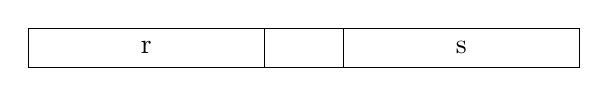
\begin{tikzpicture}
        \def \rectheight{0.5}

        % Draw the first rectangle
        \draw (0,0) rectangle (3,\rectheight);
        \node at (1.5,\rectheight / 2) {r};
        
        % Draw the middle rectangle
        \draw (3,0) rectangle (4,\rectheight);
        
        % Draw the third rectangle
        \draw (4,0) rectangle (7,\rectheight);
        \node at (5.5,\rectheight / 2) {s};
    \end{tikzpicture}
    \label{fig:vqgan_conditional_generation}
\end{figure}


After the two-phase training is finished, the transformer is used to predict a sequence $s$ which is sequence of indices to code vectors. Each token $s_i$ corresponds to an index in the codebook. So a code vector is autoregressively predicted based on the previous tokens $s_{<i}$, which provides the necessary embeddings $z_q$ for image synthesis: 

\[ p(s) = \prod_{i} p(s_i | s_{<i}) \]

To involve conditioning information $c$ such as text, images, depth map, semantic layout or pose, then a new VQ-GAN model is trained on each kind of conditioning modal, and the model obtain a new codebook $Z_c$ (which are the representation $r$ of $c$). Then, this representation is prepended to $s$ (see figure \ref{fig:vqgan_conditional_generation}) which restricts the computation of the negative log-likelihood to entries $p(s_i | s_{<i}, r)$.








\subsection{Sliding window attention technique for generating high-resolution images}

\begin{figure}[h]
    \centering
    \includegraphics[width=0.6\textwidth]{images/vqgan_sliding_attention.png}
    \caption{Sliding window attention technique proposed in the paper \cite{vqgan}.}
    \label{fig:vqgan_sliding_window}
\end{figure}

\textbf{The problem}: the attention mechanism in transformers requires quadratic computation for the number of tokens, because each token requires attention to all other tokens in the sequence (in the paper the sequence is limited to 256 tokens). Therefor they decided to use a sliding window attention mechanism to reduce the computational cost.

\textbf{Sliding window attention technique}: to solve this problem, they work patch-wise and crop input images to match the maximum token count in the transformer module, so the transformer works on the window context only, instead the entire image, which reduces the token count required.

In figure \ref{fig:vqgan_sliding_window}, the output image is divided into patches of $16\times 16$  the transformer is able to autoregressively predict the next token (code vector) $s_i$ based on the previous tokens $s_{<i}$ (the window context).


\textbf{Sampling}: to sample images, they also work patch-wise and the transformer autoregressively predicts the next token based on the window context (figure \ref{fig:vqgan_sliding_window}).
